\newpage
\section{Part IV – State estimation}
In this section an observer is developed in order to estimate the non-measured states instead of using numerical differentiation.
%-------------------------------------------------
% PROBLEM 1 - STATE SPACE FORMULATION
%-------------------------------------------------
\subsection{Problem 1 - State space formulation}
Derivation of state-space formulation of the system on the form:
\begin{equation}\label{eq:state space}
    \begin{array}{l}
    \dot x = Ax + Bu
    & y = Cx
\end{array}
\end{equation}

where;
\begin{equation}
x = \left[ {\begin{array}{*{20}{c}}
{\tilde p}\\
{\dot \tilde p}\\
{\tilde e}\\
{\dot \tilde e}\\
{\tilde \lambda }\\
{\dot \tilde \lambda }
\end{array}} \right] \textrm{,} \quad  u = \left[ {\begin{array}{*{20}{c}}
{{{\tilde V}_s}}\\
{{{\tilde V}_d}}
\end{array}} \right] \textrm{and} \quad y = \left[ {\begin{array}{*{20}{c}}
{\tilde p}\\
{\tilde e}\\
{\tilde \lambda }
\end{array}} \right]
\end{equation}

By using the equations (\ref{subeq1}) -  (\ref{eq:Travel_ddot}) we obtained the derived state-space formulation:

\begin{equation}
    \dot{x}=\left[{\begin{array}{*{20}{c}}
    {\dot{\tilde p}}\\
    {\ddot{\tilde p}}\\
    {\dot{\tilde e}}\\
    {\ddot{\tilde e}}\\
    {\dot{\tilde \lambda }}\\
    {\ddot {\tilde \lambda} }
    \end{array}} \right] = \left[ {\begin{array}{*{20}{c}}
    0&1&0&0&0&0\\
    0&0&0&0&0&0\\
    0&0&0&1&0&0\\
    0&0&0&0&0&0\\
    0&0&0&0&0&1\\
    {{K_3}}&0&0&0&0&0
    \end{array}} \right]\left[ {\begin{array}{*{20}{c}}
    {\tilde p}\\
    {\dot {\tilde p}}\\
    {\tilde e}\\
    {\dot {\tilde e}}\\
    {\tilde \lambda }\\
    {\dot {\tilde \lambda} }
    \end{array}} \right] + \left[ {\begin{array}{*{20}{c}}
    0&0\\
    0&{{K_1}}\\
    0&0\\
    {{K_2}}&0\\
    0&0\\
    0&0
    \end{array}} \right]\left[ {\begin{array}{*{20}{c}}
    {{{\tilde V}_s}}\\
    {{{\tilde V}_d}}
    \end{array}} \right]
\end{equation}

\begin{equation}
    \textbf{y} = \left[ {\begin{array}{*{20}{c}}
    1&0&0&0&0&0\\
    0&0&1&0&0&0\\
    0&0&0&0&1&0
\end{array}} \right]\textbf{x}
\end{equation}

%-------------------------------------------------
% PROBLEM 2 - Observability
%-------------------------------------------------

\subsection{Problem 2 - Observer}
Considering a system of the form:
\begin{equation}
    \dot {\hat x} = A\hat x + Bu + L(y - C\hat x)
\end{equation}

\begin{equation*}
    \dot {\hat x} = \left[ {\begin{array}{*{20}{c}}
    0&1&0&0&0&0\\
    0&0&0&0&0&0\\
    0&0&0&1&0&0\\
    0&0&0&0&0&0\\
    0&0&0&0&0&1\\
    {{K_3}}&0&0&0&0&0
    \end{array}} \right]\hat x + \left[ {\begin{array}{*{20}{c}}
    0&0\\
    0&{{K_1}}\\
    0&0\\
    {{K_2}}&0\\
    0&0\\
    0&0
    \end{array}} \right]u + L\left( {y - \left[ {\begin{array}{*{20}{c}}
    1&0&0&0&0&0\\
    0&0&1&0&0&0\\
    0&0&0&0&1&0
    \end{array}} \right]\hat x} \right)
    \end{equation*}

\textbf{Estimator MATLAB-script:}
\begin{lstlisting}
%Observability
Ob = obsv(A_s,C_s);
Orank = rank(Ob);

%Observer
es = eig(A_i-B_i*K_i);
r0 = max(abs(es));

%Radial multiplier & sector
fr = 7.5; 
phi = pi/4;
r = r0*fr;

spread= -phi:(2*phi/(5)):phi;
poles = -r *exp(1j*spread);

%Gain matrix L
L_0 = place((A_s)', (C_s)', poles);
L_s = L_0';     
\end{lstlisting}

Using the \textbf{Estimator MATLAB-script0}, we find that $\mathbf{\math\mathcal{O}}$ has full rank which implies that the system is observable. By computing the eigenvalues for $A-BK$ we find the most negative pole to be $-0.3815+0i$, which we want to multiply with $fr$ to obtain our eigenvalues for the observer.

As a thumb-rule, placing the new poles 5-10 times larger than the old ones, thus $fr = \frac{10+5}{2}=7.5$. Then we multiply this with $r$ placing 6 poles with an angle of $\phi$ between them. The pole-placements determines the gain matrix $L_s$ through line [18] and [19] in the script.

Pole-placement is a method for placing the closed-loop-poles in pre-determined locations in the s-plane. Placing poles is desirable because the location of the poles determines the eigenvalues of the system, which again controls the characteristics of the response of the system. Having the poles placed in the left-half-plane is the desirable case. 
\newpage
\renewcommand\labelitemi{\tiny$\bullet$}
\textbf{Considerations when placing poles:}
\begin{itemize}
\item Close spacing of eigenvalues results in sluggish response and a requirement of large input.
\item Large $\sigma$ results in fast response and requirement of large input.
\item Large $r$ results in fast response and requirement of large input.
\item Large $\theta$ results in greater overshoot.
\end{itemize}

\begin{figure}[!htb]
    \centering
    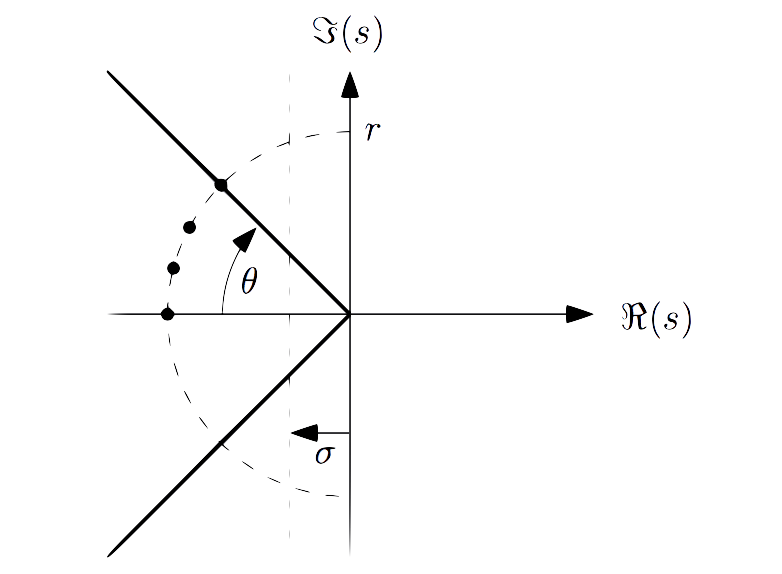
\includegraphics[scale=0.5]{images/poleplacement}
    \caption{Poleplacement}
    \label{poles}
\end{figure}

Reflecting over the pole-placement, the hardware specifications have to be accounted for. The signals for inputs and outputs have maximum values, which causes a maximum reasonable limit for $\sigma$. Increasing $\sigma$ further would maximize the output-values of the signals. By this there will be no middle-values, the controller requires larger values than what is actually possible, resulting in vibrations and oscillations.
\newpage
\begin{figure}[!htb]
    \centering
    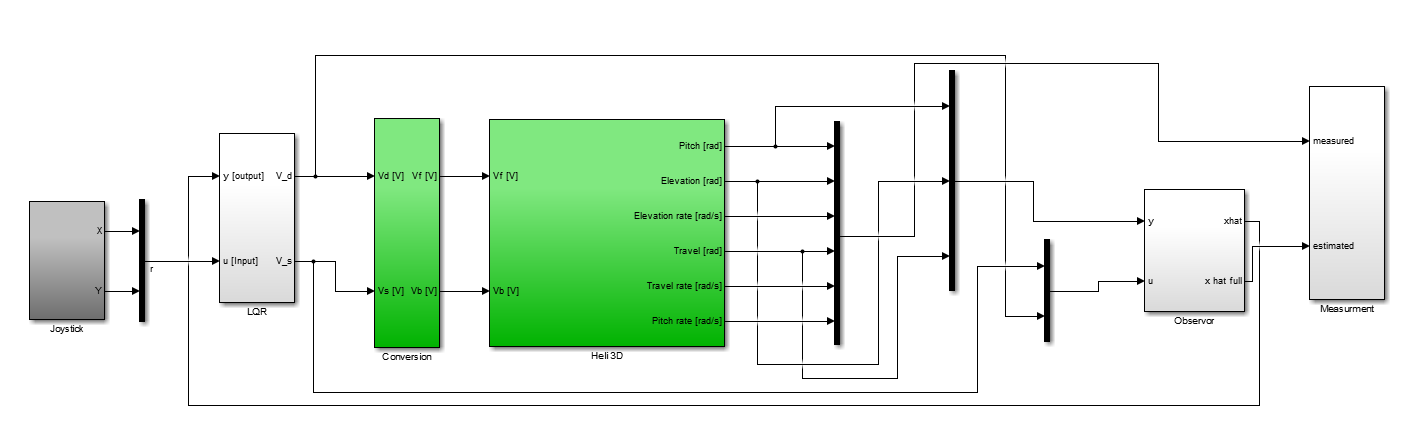
\includegraphics[scale=0.4]{images/Estimator_LQR}
    \caption{Observer - SimuLink Model}
    \label{Observer}
\end{figure}

\begin{figure}[!htb]
    \centering
    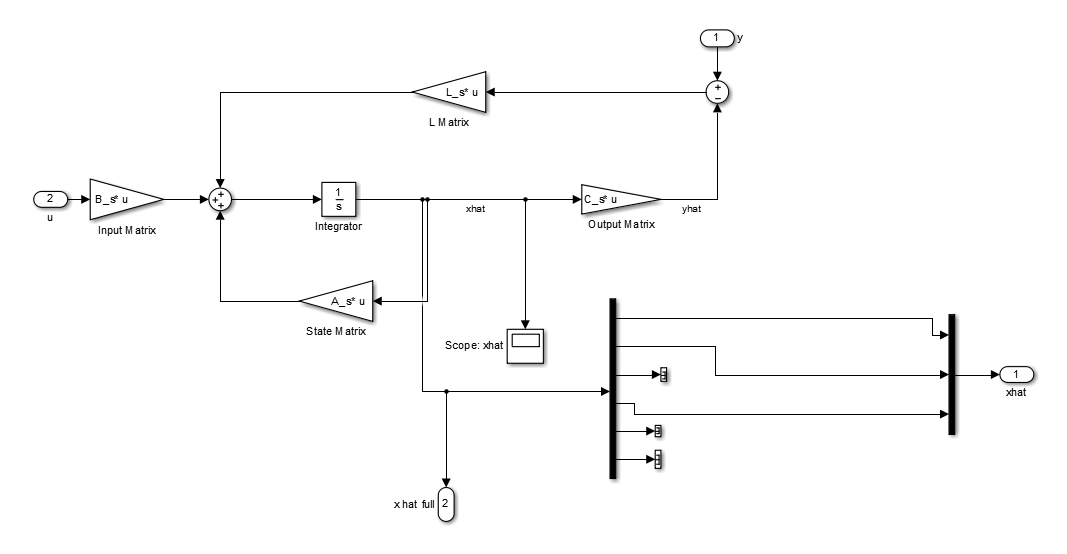
\includegraphics[scale=0.5]{images/Observator1}
    \caption{Observer block}
    \label{poles}
\end{figure}

\newpage
\subsection{Problem 3 - Measurement & Observability}

In this section we are going to develop a linear observer based on the measurement vector $\textbf{y}$ and plot the measured states together with the estimated states. The measurement vector is given as:
\begin{equation}
    y = \left[ {\begin{array}{*{20}{c}}
    {\tilde e}\\
    {\tilde \lambda }
\end{array}} \right]
\end{equation}

The following MATLAB-script were used to calculate the observability of the different measured states:
\textbf{Estimator MATLAB-script:}
\begin{lstlisting}
%Pole-placement Problem 4.3
fr_3 = 1;
phi_3 = pi/3.5;
r_3 = r0*fr_3;
spread_3 = -phi_3:(phi_3/2.5):phi_3;
prob_3_poles = -r_3 * exp(1i * spread_3);

%Matrices
C_1 = [0 0 1 0 0 0;0 0 0 0 1 0];
C_2 = [1 0 0 0 0 0;0 0 1 0 0 0];

Ob_1 = rank(obsv(A_s,C_1)); %Observable
Ob_2 = rank(obsv(A_s,C_2)); %Not observable

L_1_s = )place((A_s)', (C_s)', poles))';
\end{lstlisting}

Using the given measurement vector, new matrices for C and L had to be calculated in \textbf{MATLAB}.

\textbf{Determinations:}

\begin{equation*}
    y = \left[ {\begin{array}{*{20}{c}}
    {\tilde e}\\
    {\tilde \lambda }
    \end{array}} \right] \to rank({\mathbf{\math\mathcal{O}}}) = 6
\end{equation*}
The observability matrix has rank 6 $\to$ The system is observable.

Analysing the performance of the new observer, we could clearly see that the pitch and pitch rate had poor performane, due to many factors, among that the pitch is the unmeasured state and relies only on the model. 


\begin{equation*}
    y = \left[ {\begin{array}{*{20}{c}}
    {\tilde p}\\
    {\tilde e}
    \end{array}} \right] \to rank({\mathbf{\math\mathcal{O}}}) = 4
\end{equation*}
The observability matrix has rank 4 $\to$ The system is \underline{not} observable.\\

The state estimate for $\tilde {\lambda}$ has a second-derived ${\ddot {\tilde {\lambda}}}$ that is dependant of ${\tilde p}$, making it rather hard to both estimate and measure. It can still be done, if the poles are placed correctly. The model itself, is linearised, thus the state estimator is prone to linearization errors. 



\newpage
\subsection{Graphs}


%%ADDING GRAPHS!!!!
\begin{figure}[!htb]
    \centering
    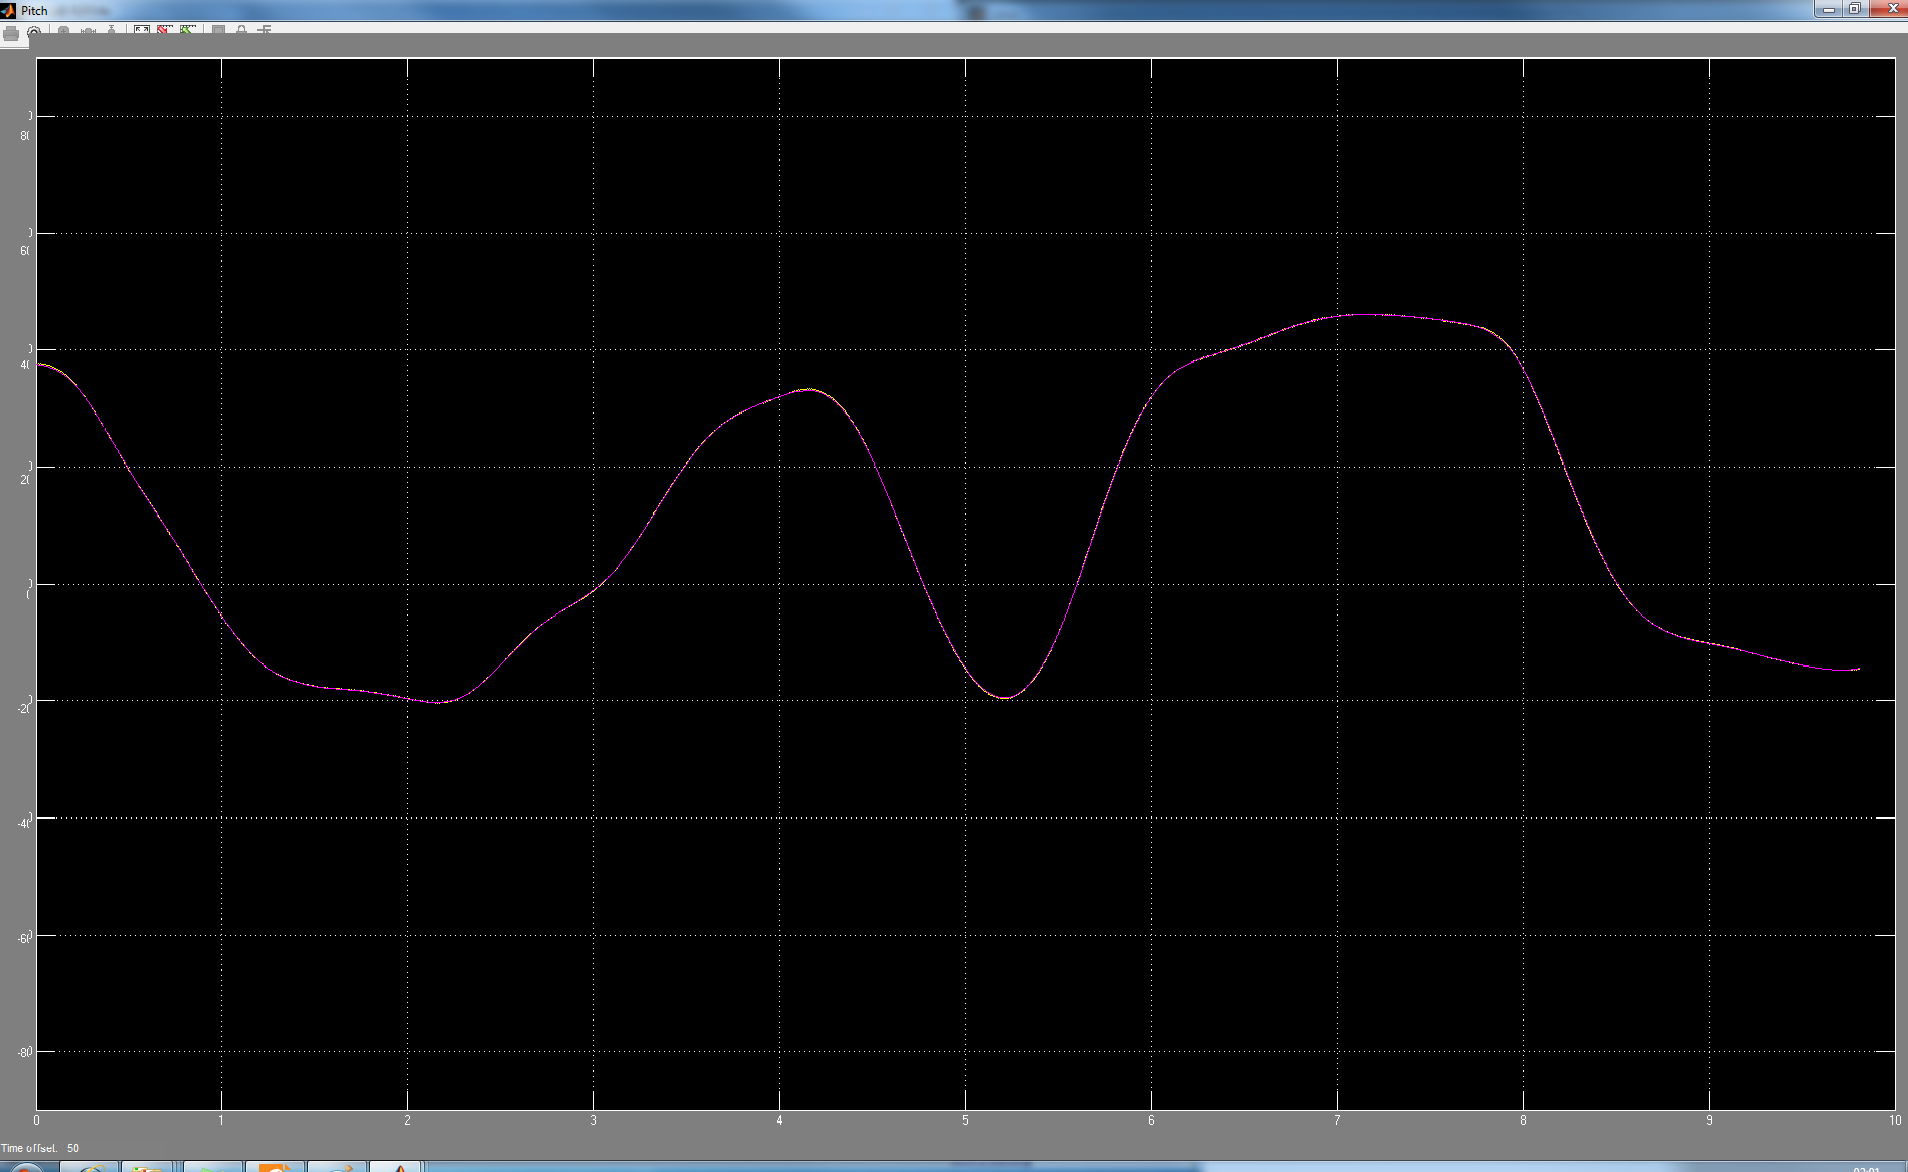
\includegraphics[scale=0.25]{images/pitch}
    \caption{Pitch Estimator}
   
\end{figure}
\begin{figure}[!htb]
    \centering
    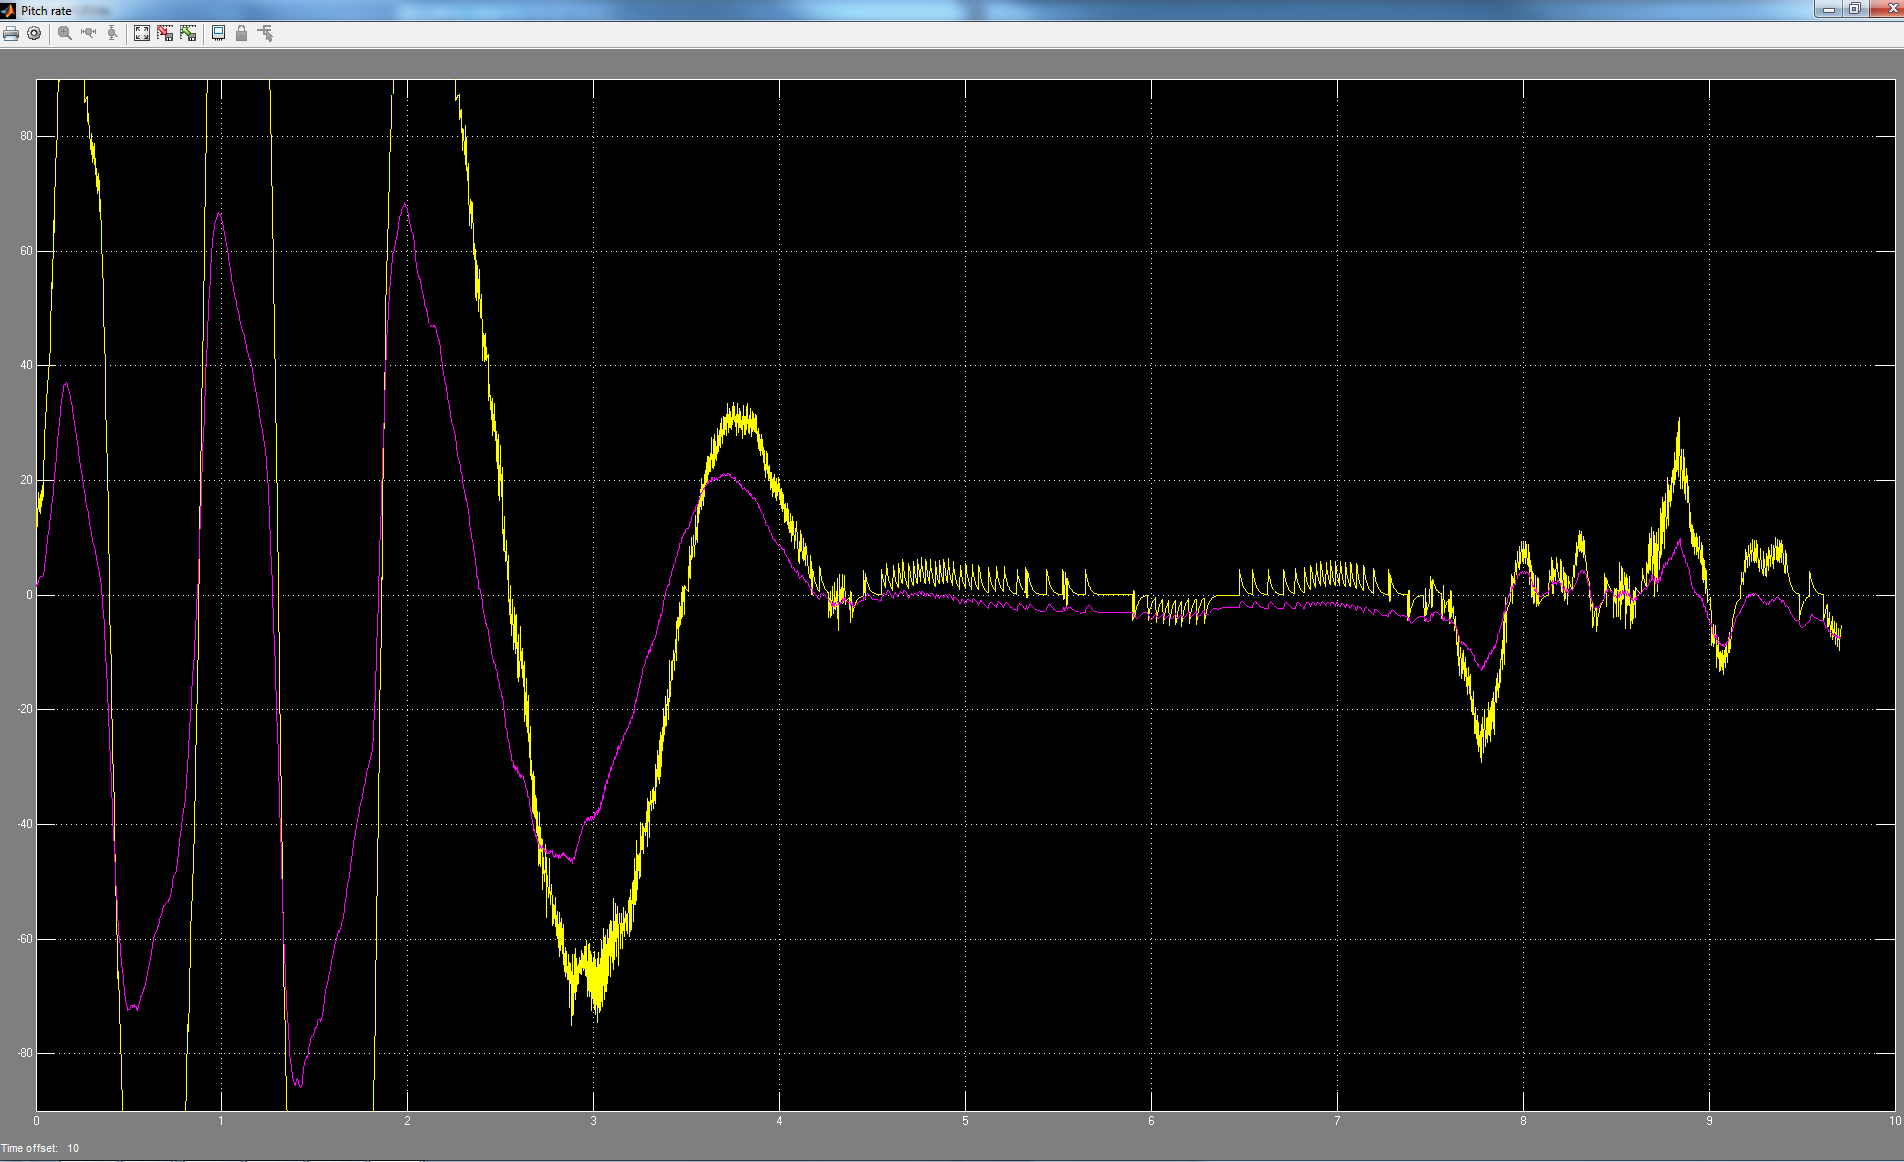
\includegraphics[scale=0.25]{images/pitchrate}
    \caption{Pitch rate Estimator}

\end{figure}
\begin{figure}[!htb]
    \centering
    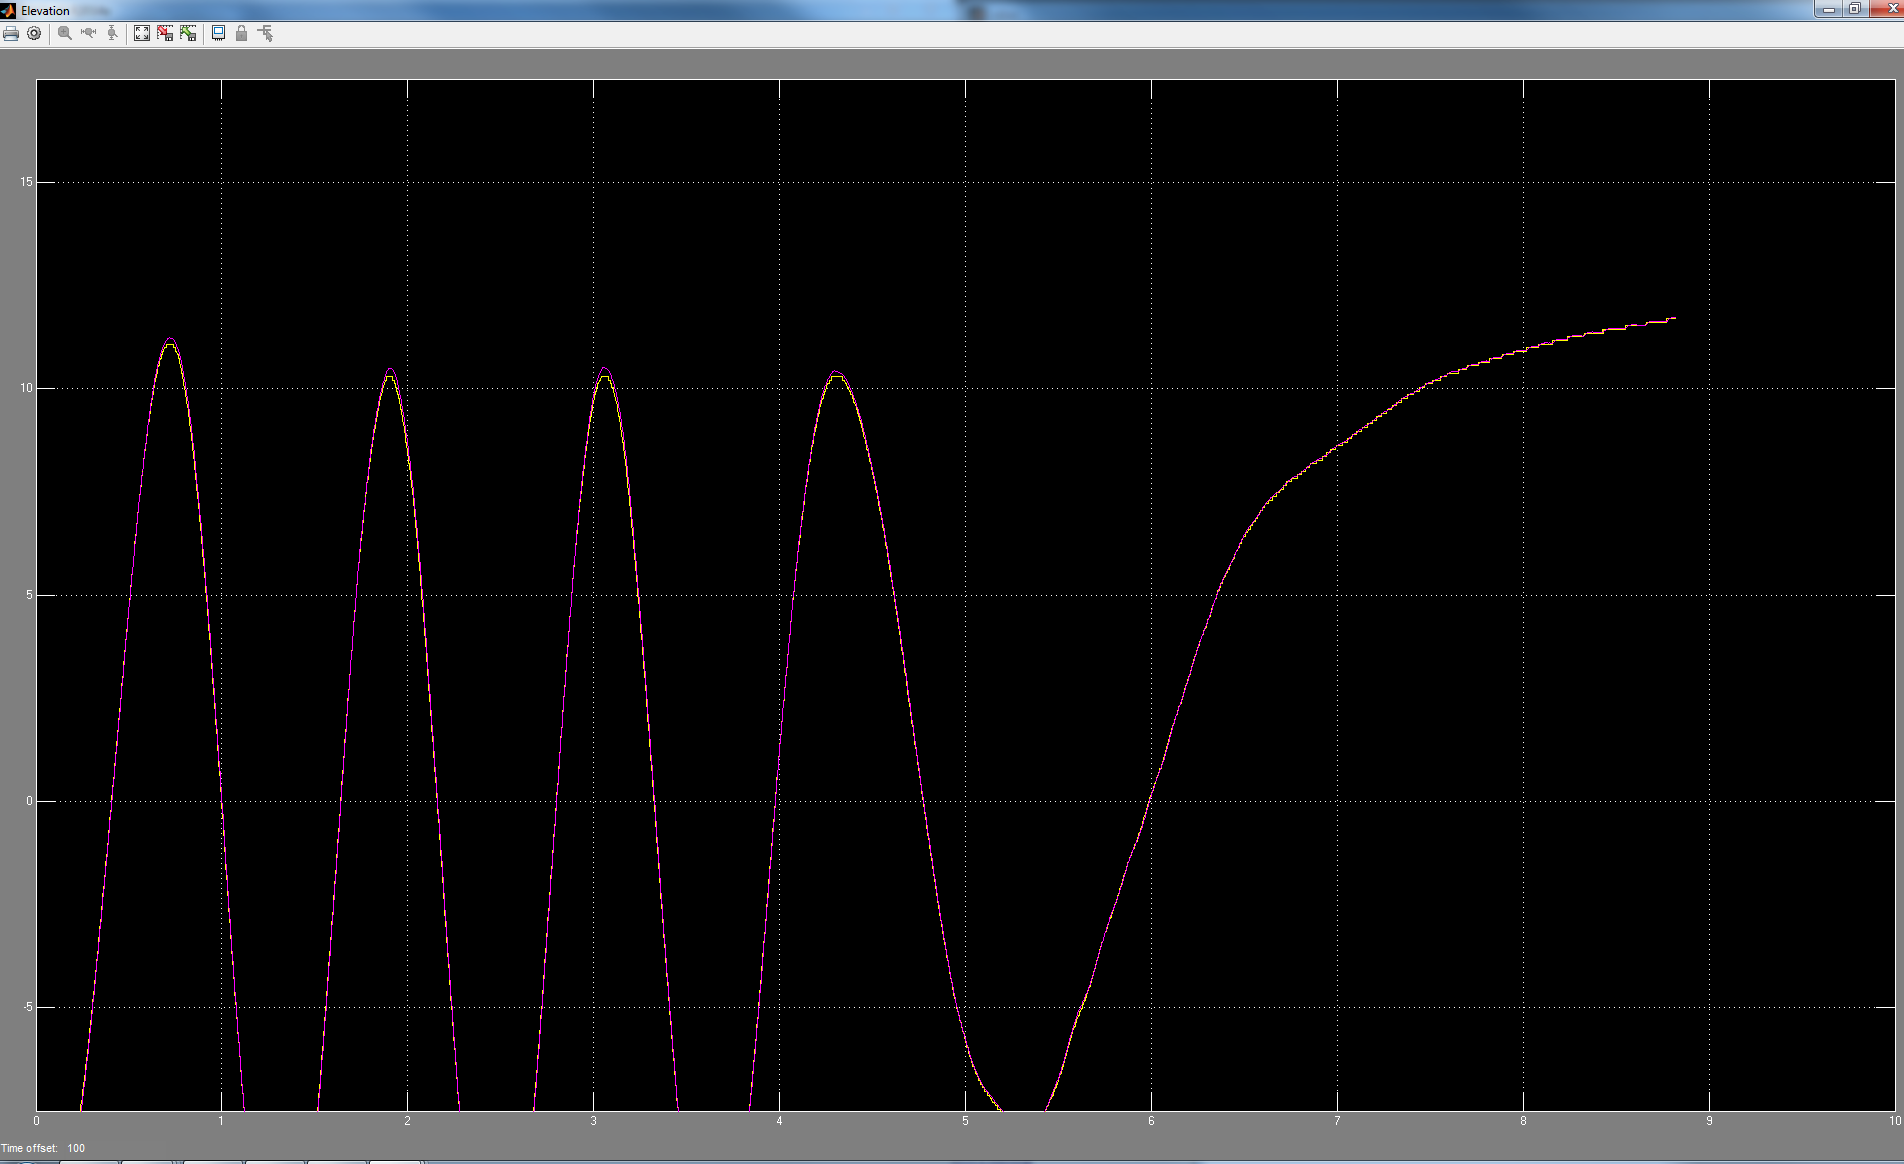
\includegraphics[scale=0.25]{images/elevation}
    \caption{Elevation Estimator}

\end{figure}
\begin{figure}[!htb]
    \centering
    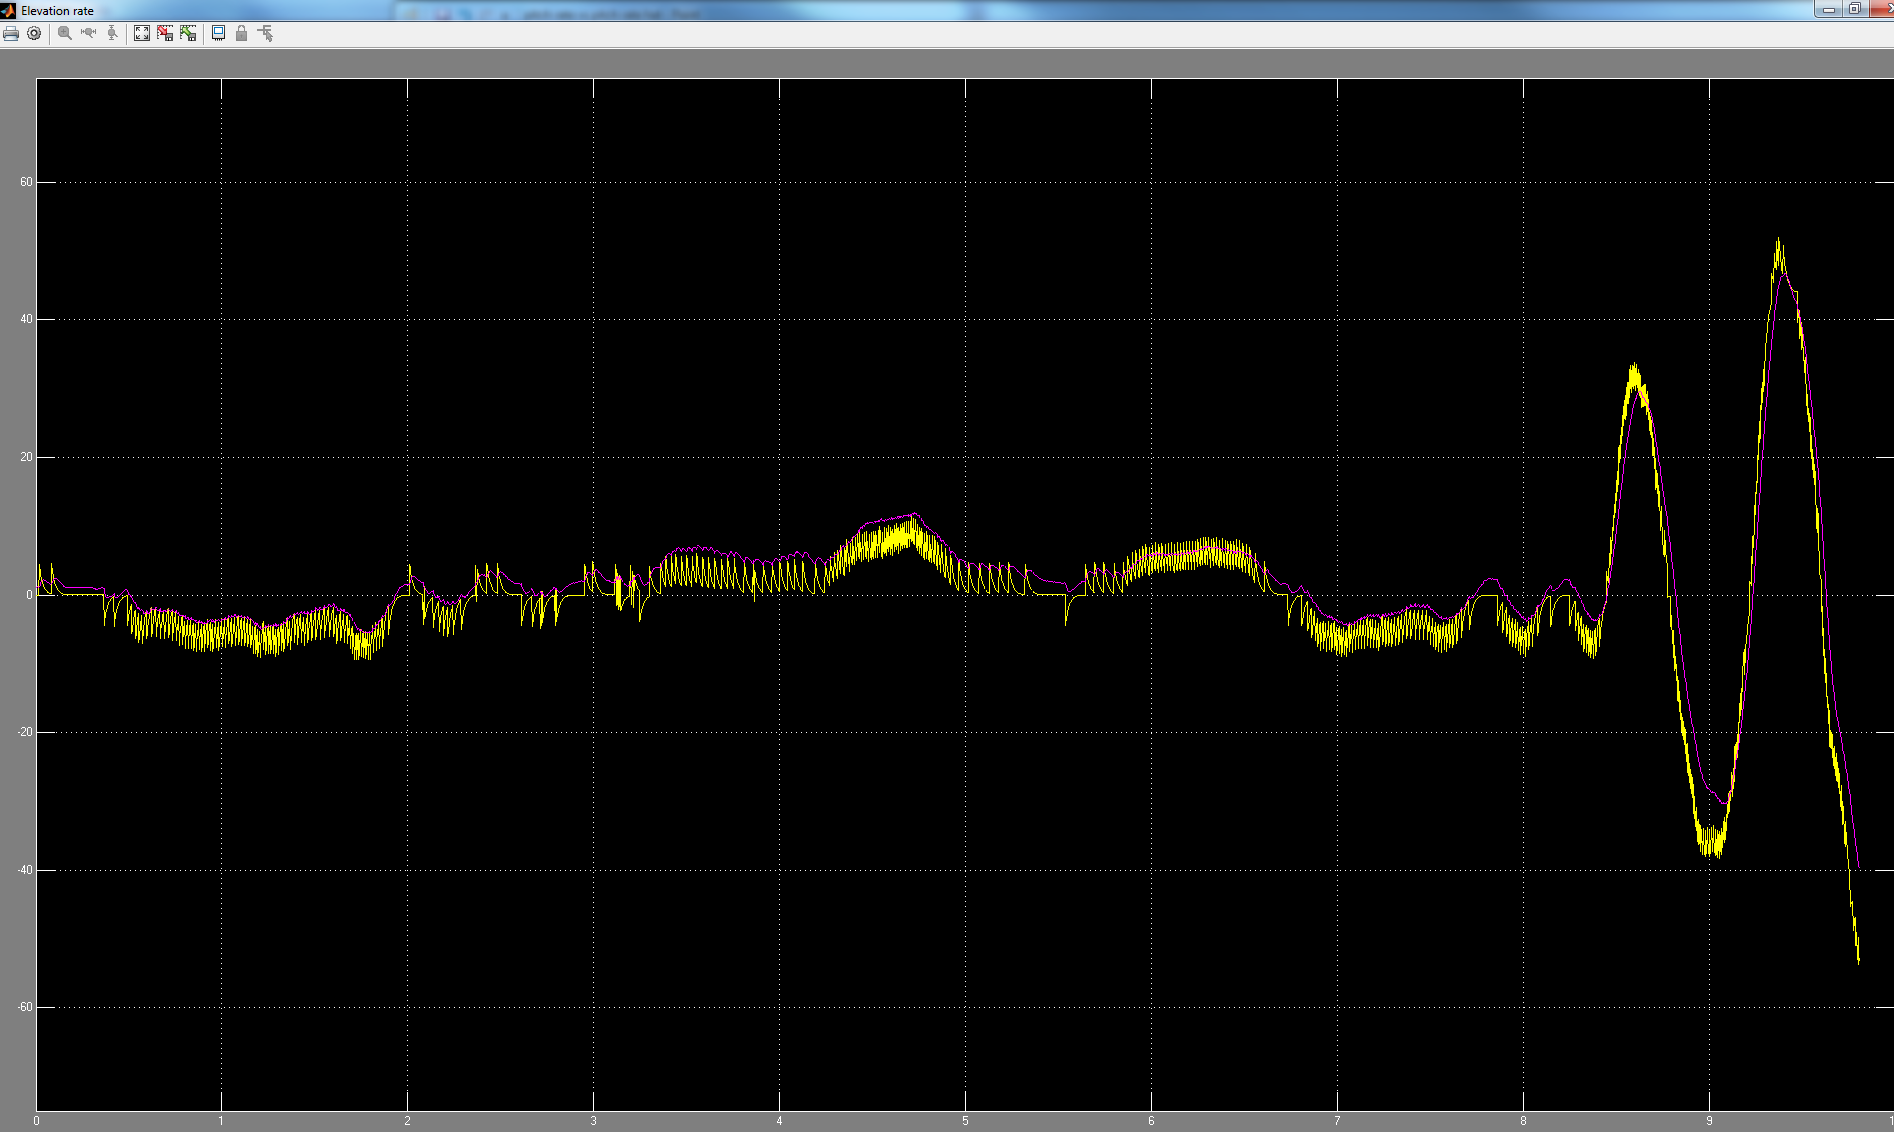
\includegraphics[scale=0.25]{images/elevationrate}
    \caption{Elevation rate Estimator}
\end{figure}


\begin{figure}
    \centering
    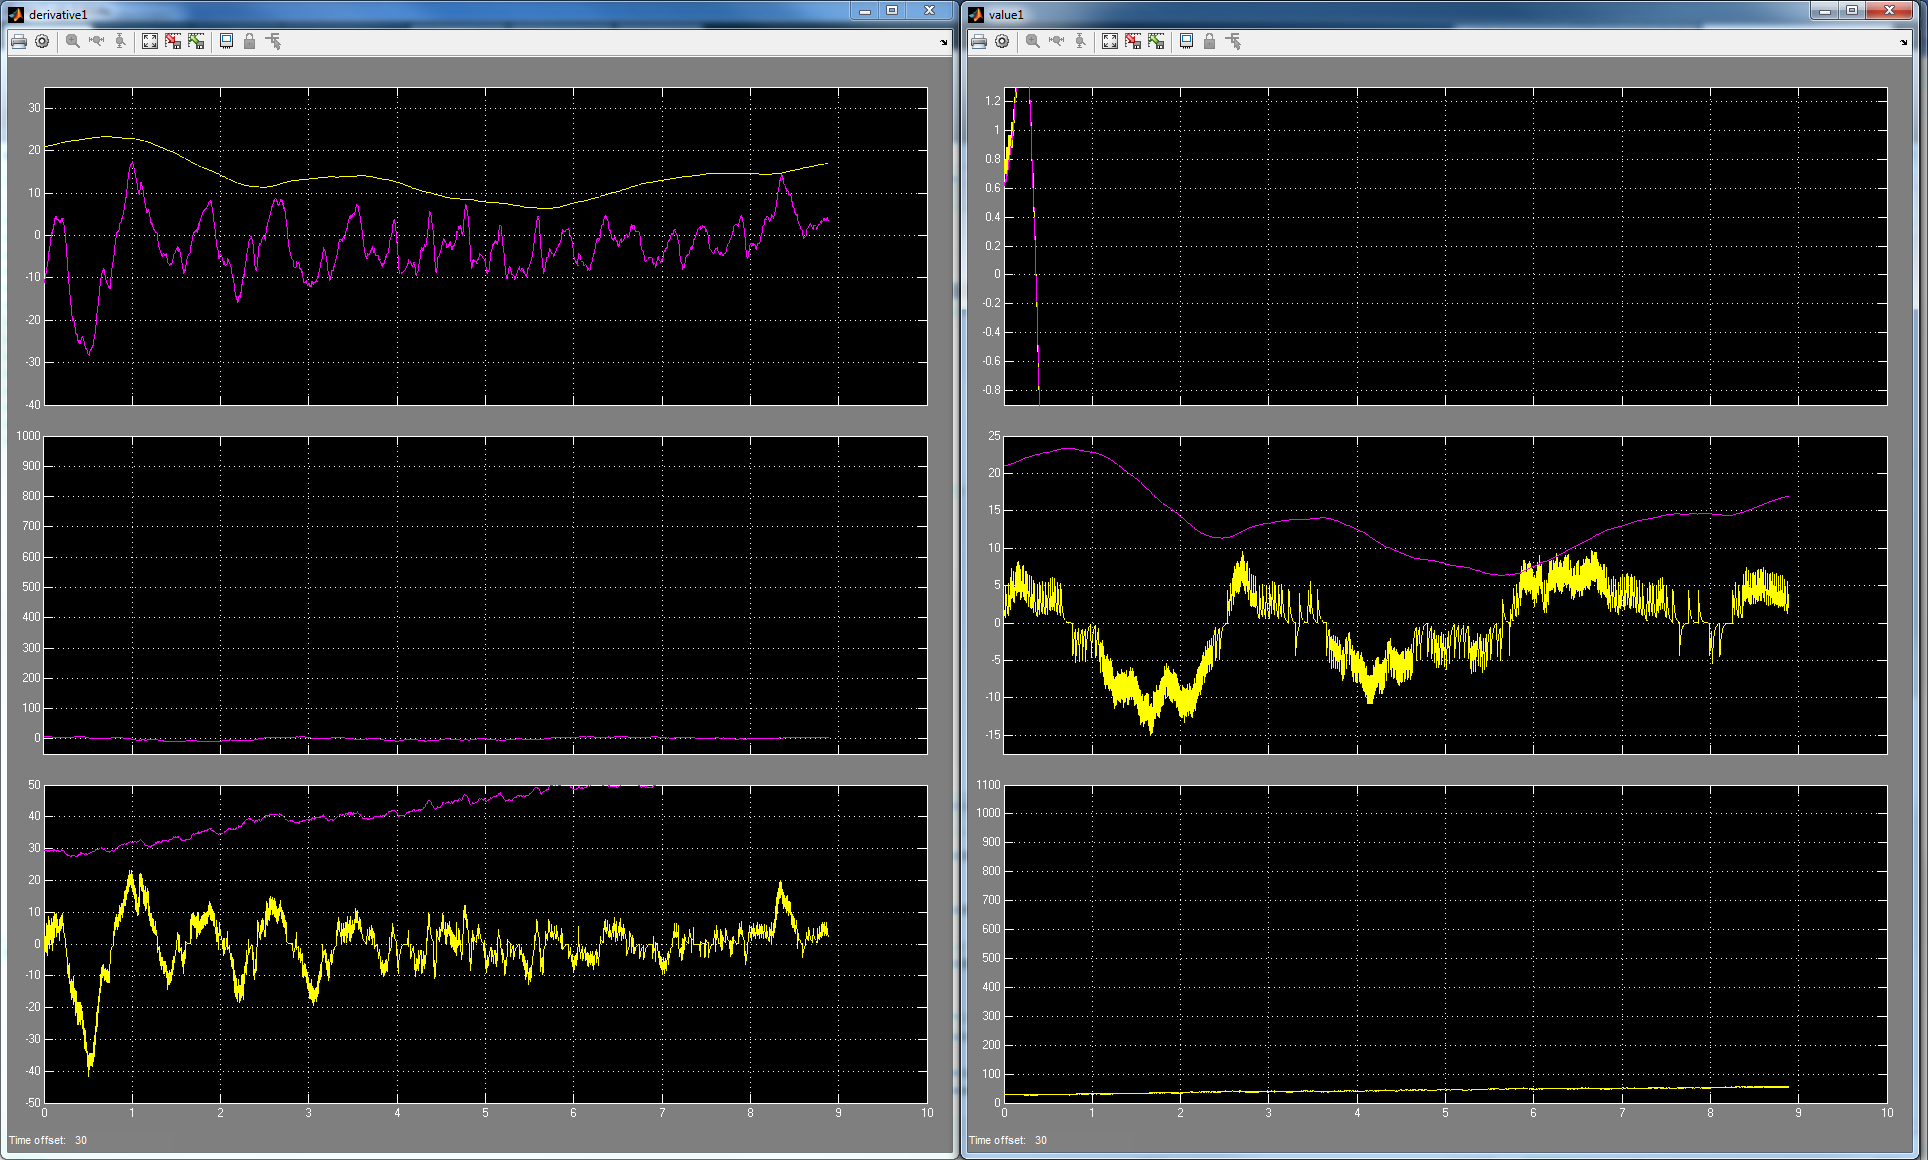
\includegraphics[scale=0.25]{images/all-states}
    \caption{All states Estimator}
\end{figure}

